\chapter{Project plan}
The project starts at August 18th, 2015.
We expect to deliver it on March 25th, 2016.
For our project planing, we divide our work into 4 phases.
\begin{enumerate}
\item Plan and research (18/08/15 -- 30/10/15) \hfill \\
The first phase was to gather user's requirements by interviewing.
We interviewed with \gls{ic}'s vice dean because he is a client who came up with this project.
Then, we moved on to interviewing \gls{ic}'s employees asking about document related problem they encountered.
Next, we discussed about software tools that solve the problem.
\item Design and architecture (29/09/15 -- 23/11/15) \hfill \\
On the second phase, we designed the software architecture.
The architecture is the core of how software must behave, also to get an overview of system interaction.
Then, we designed a \gls{gui} of this system.
\item System implementation (7/12/15 -- 22/02/16) \hfill \\
This phase began writing source codes based on user requirements, designed architecture, and technical specification.
Later on, we connected each system's components together.
\item Testing (19/02/16 -- 07/03/16) \hfill \\
This phase ensured that systems ran correctly with user and system requirements.
We also conducted user acceptance testing.
Then, We evaluated testing result.
If the result were satisfying, we would deploy the system to \gls{ic}'s server.
\end{enumerate}

\begin{landscape}
\begin{figure}
\centering
\caption{Project's schedule shown as Gantt chart}
\label{fig:project-schedule}
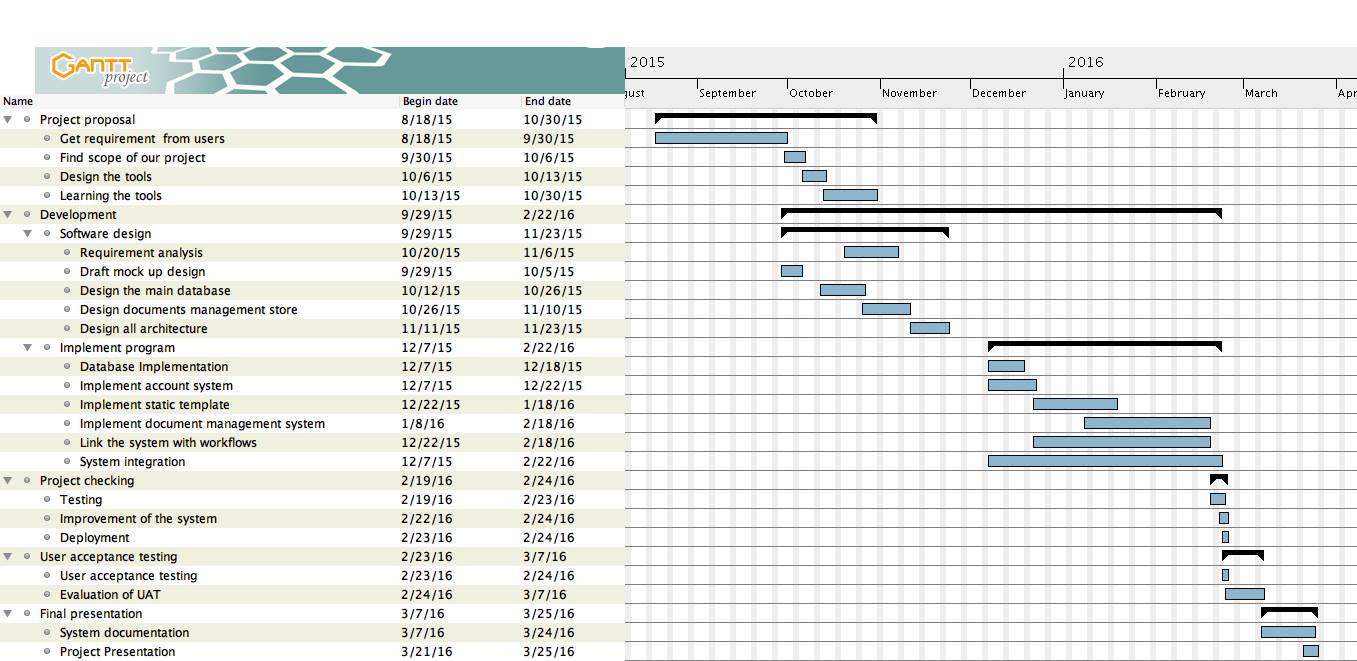
\includegraphics[scale=0.4]{res/project_plan}
\end{figure}
\end{landscape}